\chapter{Hồi quy trọng số địa lý (GWR)}
\label{ch:M6L3LessonNotes}

\section*{Lesson Notes}

MODULE 6 \textbar{} BÀI 3

{\small
\begin{longtable}[]{@{}
  >{\raggedright\arraybackslash}p{(\columnwidth - 2\tabcolsep) * \real{0.5000}}
  >{\raggedright\arraybackslash}p{(\columnwidth - 2\tabcolsep) * \real{0.5000}}@{}}
\toprule\noalign{}
\endhead
\bottomrule\noalign{}
\endlastfoot
\textbf{Thời gian đọc} & 2 giờ \\
\textbf{Kiến thức nền} & thống kê cơ bản, hồi quy tuyến tính, Python \\
\textbf{Từ khóa} & Phân tích không gian, hồi quy, GWR, tính không đồng nhất không gian, hàm nhân (kernel) \\
\end{longtable}
}

\begin{center}\rule{0.5\linewidth}{0.5pt}\end{center}

\emph{Bài học này giới thiệu hồi quy trọng số địa lý (GWR) như một cách đơn giản, trực quan để mô hình hóa dữ liệu có tính không đồng nhất không gian. Chúng ta tìm hiểu nền tảng lý thuyết của GWR, bắt đầu từ động cơ ra đời và cách GWR mở rộng hồi quy tuyến tính truyền thống để xét đến tính không đồng nhất không gian. Ở nửa sau của notebook, chúng ta thực hành với các minh họa và một ví dụ dữ liệu thực tế, nhằm bổ sung cho lý thuyết những kỹ năng cần thiết để áp dụng GWR trong thực tế.}

\begin{lstlisting}[language=Python,escapeinside={(*@}{@*)}]
import numpy as np
import matplotlib.pyplot as plt
import seaborn as sns
sns.set()
\end{lstlisting}

\section{Hồi quy trọng số địa lý (GWR)}

Hồi quy trọng số địa lý (GWR) là phần mở rộng của hồi quy tuyến tính truyền thống, có xét đến \textbf{tính không đồng nhất không gian (spatial heterogeneity)} trong quan hệ giữa các biến. Phương pháp này cho phép các hệ số thay đổi theo vị trí địa lý, nhờ đó nắm bắt được sự khác biệt về quan hệ giữa các điểm khác nhau trong không gian. Nói ngắn gọn, đây là hồi quy tính đến vị trí của biến phụ thuộc trên bản đồ và giả định quan hệ của nó với các biến độc lập hoàn toàn có thể khác với quan hệ tại một điểm khác trên bản đồ.

Để đạt được điều đó, khung GWR thực hiện số hồi quy tuyến tính bằng số điểm dữ liệu trên bản đồ. Mỗi hồi quy là một hồi quy tuyến tính có trọng số (WLS), trong đó trọng số đóng vai trò hệ số suy giảm: điểm càng xa nơi thực hiện WLS thì càng ít quan trọng.

Điều đầu tiên cần thấy là các hệ số của GWR không còn là hằng số trên toàn bản đồ. Ngược lại, mỗi điểm có một bộ hệ số riêng, cùng với hệ số chặn và sai số. Đây chính là điểm mạnh của khung này: cho phép hiểu thấu đáo cách quan hệ giữa các biến thay đổi theo không gian.

Trước hết ta viết hồi quy tuyến tính truyền thống. Trong bối cảnh GWR, hồi quy này được gọi là \emph{"toàn cục (global)"} vì giả định các hệ số toàn cục (không đổi). Công thức hồi quy tuyến tính (LR):

\textbf{Hồi quy tuyến tính truyền thống}

\[
y_{i} = \beta_{0} + \sum_{k = 1}^{p} \beta_{i} \cdot x_{ik} + \epsilon_{i}
\]

trong đó

\begin{itemize}
\item
  \(y\) là biến phụ thuộc
\item
  \(\beta_{i}\) là các hệ số (giả định không đổi trên mọi quan sát)
\item
  \(x_{ik}\) là \(k\) biến độc lập và
\item
  \(\epsilon_{i}\) là các sai số
\end{itemize}

\textbf{Hồi quy trọng số địa lý}

Trong GWR, ta cho phép các hệ số thay đổi theo vị trí; do đó chúng trở thành hàm của không gian: \(\beta(u, v)\), với \((u,v)\) là tọa độ.

\[
y_{i} = \beta_{0}(u_{i}, v_{i}) + \sum_{k=1}^{p}\beta_{k}(u_{i}, v_{i})x_{ik} + \epsilon{i}
\]

Ký hiệu trên che giấu một bất tiện quan trọng: mỗi điểm trên bản đồ chỉ có một (hoặc vài) quan sát, nên không thể ước lượng đáng tin cậy các hệ số tại từng điểm bằng ước lượng OLS. Để xử lý, ta dùng lược đồ trọng số không gian mã hóa ảnh hưởng của các điểm lên điểm đang xét. Đương nhiên, điểm ở xa được gán trọng số nhỏ hơn điểm ở gần. Kết quả là ma trận trọng số đường chéo \(W\) chứa các giá trị từ 0 đến 1.

Việc dùng ma trận trọng số có nghĩa là với mỗi điểm trên bản đồ, ta ước lượng \(\beta{i}\) bằng mọi quan sát sẵn có, được gán trọng số theo độ gần với điểm đang xét. Khi đó ước lượng hệ số được cho bởi:

\[
\hat \beta(u_{i}, v_{i}) = [X^{T} W(u_{i}, v_{i}) X]^{-1} X^{T} W(u_{i}, v_{i}) y
\]

Suy ra giá trị dự báo của mỗi quan sát là:

\[
\hat y_{i} = X_{i} [X^{T} W(u_{i}, v_{i}) X]^{-1} X^{T} W(u_{i}, v_{i}) y
\]

Nếu đặt:

\[
S_{i} = X_{i} [X^{T} W(u_{i}, v_{i}) X]^{-1} X^{T} W(u_{i}, v_{i}) \text{ and } C_{i} = [X^{T} W(u_{i}, v_{i}) X]^{-1} X^{T} W(u_{i}, v_{i})
\]

thì ma trận hiệp phương sai cục bộ \(V_{i}\) của các ước lượng tham số là:

\[
V_{i} = C_{i} C^{T}_{i} \hat \sigma^{2}
\]

trong đó \(\hat \sigma^{2}\) là độ lệch chuẩn ước lượng của số hạng sai số, được định nghĩa là:

\[
\hat \sigma^{2} = \frac{\sum (y_{i} - \hat y_{i})^{2}}{m - tr(S)}
\]

Bây giờ ta xem xét lược đồ trọng số.

\subsection{Sơ đồ trọng số (sơ đồ "mượn dữ liệu")}

Sơ đồ trọng số trong GWR còn gọi là "sơ đồ mượn dữ liệu" (data-borrowing scheme). Tên gọi này nhấn mạnh rằng sự gần nhau về không gian, tức việc mượn các quan sát lân cận, là yếu tố then chốt để ước lượng các hệ số hồi quy cục bộ.

Trọng số của mỗi quan sát được cho bởi các hàm nhân không gian (kernel). Ba hàm nhân phổ biến nhất là:

\begin{itemize}
\item
  \textbf{Hàm nhân Gaussian}:
\end{itemize}

\[
w_{ij} = \exp \left ( -\frac{d^{2}_{ij}}{2b^{2}} \right )
\]

\begin{itemize}
\item
  \textbf{Hàm nhân Bisquare}:
\end{itemize}

\[
w_{ij} = \begin{cases}
     \left ( 1 - \left ( \frac{d_{ij}}{b} \right )^{2} \right )^2 & \text{ if } d_{ij} < b \\
     0 & \text{ otherwise }
\end{cases}
\]

\begin{itemize}
\item
  \textbf{Hàm nhân mũ (Exponential)}:
\end{itemize}

\[
w_{ij} = \exp \left ( -\frac{d_{ij}}{b} \right )
\]

trong đó

\begin{itemize}
\item
  \(w_{ij}\) là trọng số của quan sát \(j\) khi ước lượng mô hình tại quan sát \(i\)
\item
  \(d_{ij}\) là khoảng cách giữa \(i\) và \(j\)
\item
  \(b\) là tham số băng thông (bandwidth), kiểm soát mức suy giảm của trọng số theo khoảng cách
\end{itemize}

\textbf{Khoảng cách}

Việc chọn thước đo khoảng cách giữa hai điểm tùy theo từng bài toán. Thông thường khoảng cách Euclid (đường thẳng giữa hai điểm) là đủ:

\[
d_{ij} = \sqrt{(u_{i} - u_{j})^{2} + (v_{i} - v_{j})^{2}}
\]

Nếu bài toán cần tính đến mạng lưới đường phố dạng ô vuông, có thể dùng khoảng cách Manhattan:

\[
d_{ij} = |u_{i} - u_{j}| + |v_{i} - v_{j}|
\]

Nếu vùng nghiên cứu rộng (độ cong Trái Đất trở nên đáng kể) và/hoặc địa hình đa dạng, đường trắc địa hay khoảng cách trắc địa có thể phù hợp hơn.

\textbf{Tham số băng thông}

Băng thông \(b\) điều tiết sự đánh đổi giữa thiên lệch (bias) và phương sai thông qua mức độ gần của các điểm dùng trong các hồi quy cục bộ. Băng thông nhỏ nhấn mạnh biến thiên cục bộ nhưng chỉ giữ ít quan sát để ước lượng tham số. Băng thông lớn có thể giảm phương sai của hệ số nhưng có thể bỏ sót đặc điểm cục bộ do bị "làm trơn quá mức" khi đưa các điểm ở xa vào phân tích. Băng thông thường được chọn bằng kiểm định chéo (CV) hoặc tiêu chí thông tin Akaike (AIC).

Hãy minh họa hình dạng các hàm nhân trong thực tế. Trong ví dụ tiếp theo, ta dùng một "bản đồ" vuông gồm \(100 \times 100 = 10,000\) quan sát. Các hình minh họa gồm cả ba hàm nhân và cho thấy khác biệt giữa khoảng cách Manhattan và Euclid. Để đơn giản, điểm quan tâm được cố định tại tâm bản đồ.

\begin{lstlisting}[language=Python,escapeinside={(*@}{@*)}]
# Figure 1
# Create a meshgrid
i_indices = np.arange(100)
j_indices = np.arange(100)
I, J = np.meshgrid(i_indices, j_indices, indexing='ij')

# Manhattan and Euclidean distances
manhattan_distance = np.abs(I - 50) + np.abs(J - 50)
euclidean_distance = np.sqrt((I - 50)**2 + (J - 50)**2)

# Kernel functions
def gaussian_kernel(D, b):
    return np.exp(- (D ** 2) / (2 * b ** 2))

def bisquare_kernel(D, b):
    return ((1 - (D / b) ** 2) ** 2) * (D < b) # Comment this line yourself

def exponential_kernel(D, b):
    return np.exp(- D / b)

# Plotting function
def plot_kernels(D, bandwidth):
    # Compute weights
    W_gaussian = gaussian_kernel(D, bandwidth)
    W_bisquare = bisquare_kernel(D, bandwidth)
    W_exponential = exponential_kernel(D, bandwidth)

    # Set up the plot
    fig, axs = plt.subplots(1, 3, figsize=(18, 6))

    # Gaussian Kernel
    sns.heatmap(W_gaussian, cmap='viridis', ax=axs[0])
    axs[0].set_title(f'Gaussian Kernel (b = {bandwidth})')

    # Bisquare Kernel
    sns.heatmap(W_bisquare, cmap='viridis', ax=axs[1])
    axs[1].set_title(f'Bisquare Kernel (b = {bandwidth})')

    # Exponential Kernel
    sns.heatmap(W_exponential, cmap='viridis', ax=axs[2])
    axs[2].set_title(f'Exponential Kernel (b = {bandwidth})')

    plt.tight_layout()
    plt.show()


# Plot the kernels using manhattan distance
for b in [10, 25, 50]:
    plot_kernels(D = manhattan_distance, bandwidth=b)
\end{lstlisting}

\begin{figure}[H]
\centering
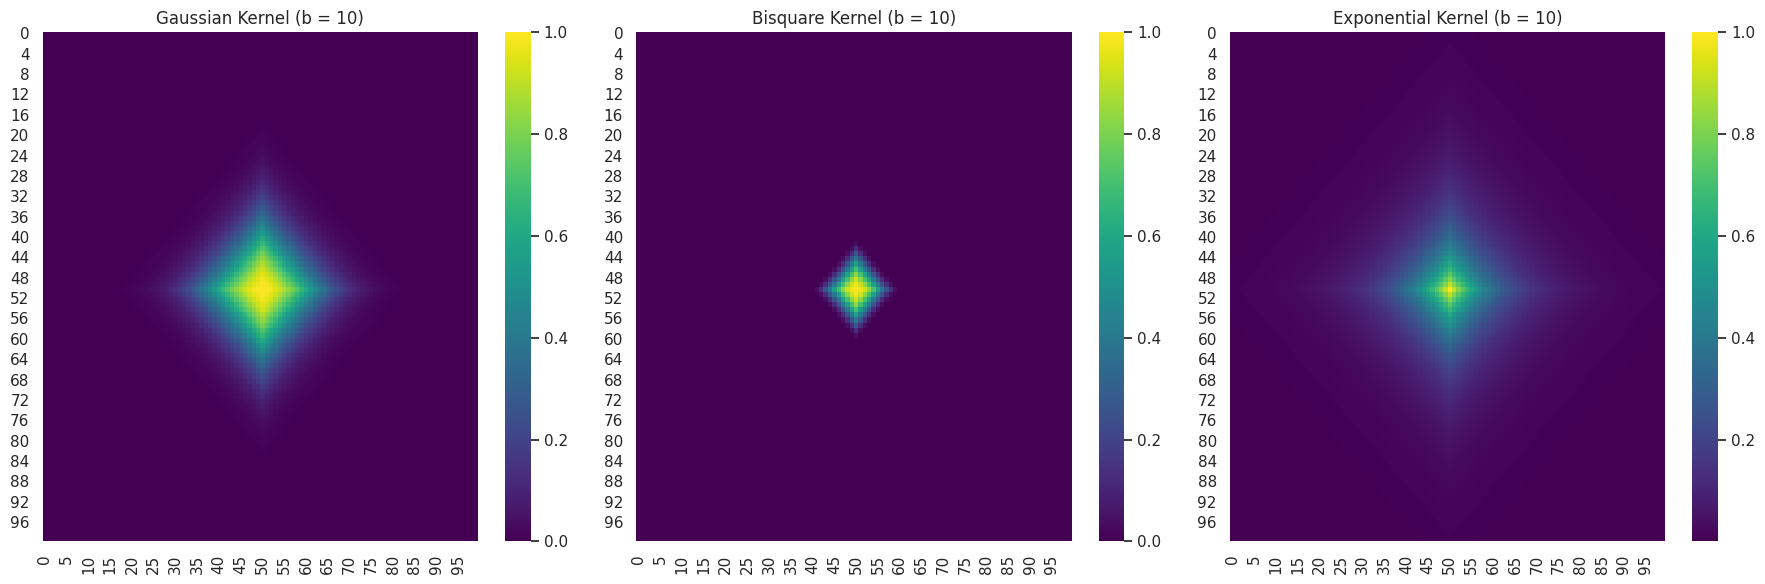
\includegraphics[width=0.85\linewidth]{gfx/m6l3_img001.png}
\par\smallskip{\small \textbf{Hình:} Hàm nhân (kernel) theo khoảng cách Manhattan, băng thông 10.}
\end{figure}

\begin{figure}[H]
\centering
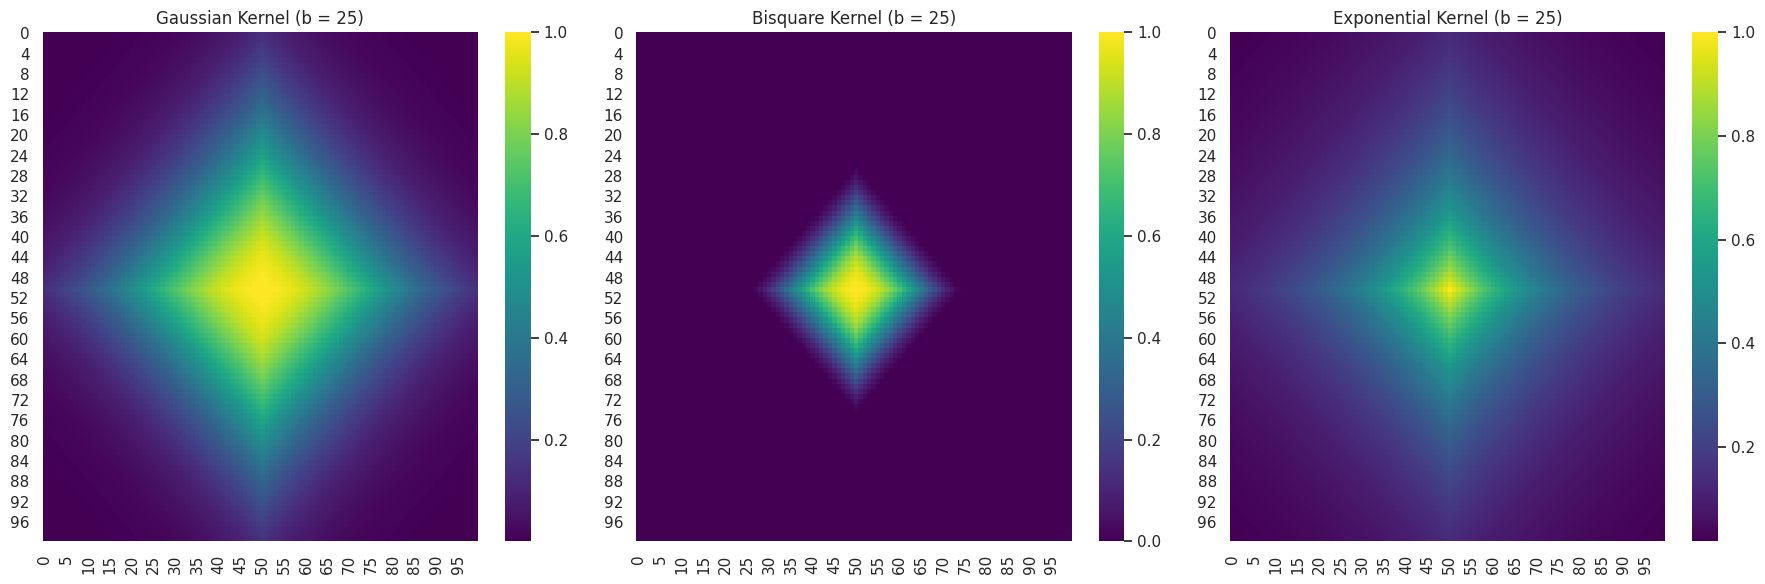
\includegraphics[width=0.85\linewidth]{gfx/m6l3_img002.png}
\par\smallskip{\small \textbf{Hình:} Hàm nhân (kernel) theo khoảng cách Manhattan, băng thông 25.}
\end{figure}

\begin{figure}[H]
\centering
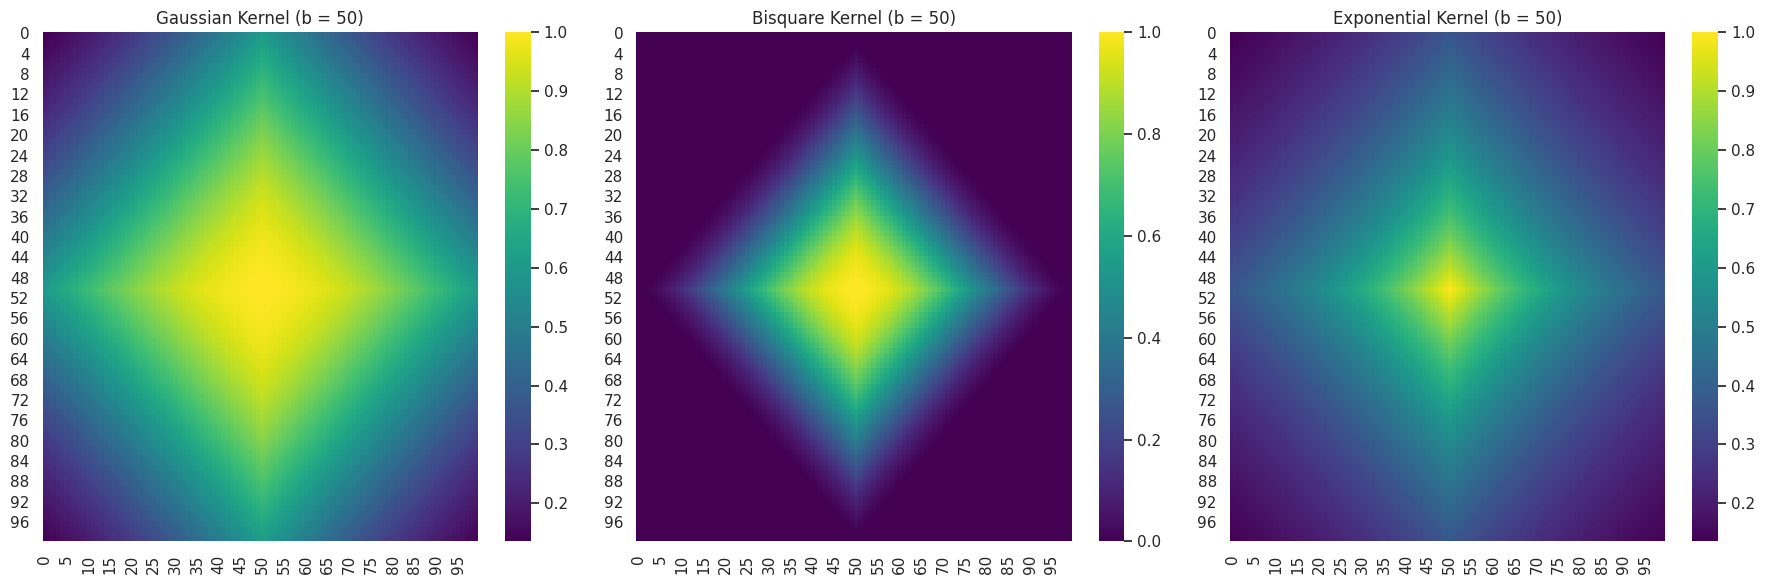
\includegraphics[width=0.85\linewidth]{gfx/m6l3_img003.png}
\par\smallskip{\small \textbf{Hình:} Hàm nhân (kernel) theo khoảng cách Manhattan, băng thông 50.}
\end{figure}

\begin{lstlisting}[language=Python,escapeinside={(*@}{@*)}]
# Figure 2
# Plot the kernels using Euclidean distance
for b in [10, 25, 50]:
    plot_kernels(D = euclidean_distance, bandwidth=b)
\end{lstlisting}

\begin{figure}[H]
\centering
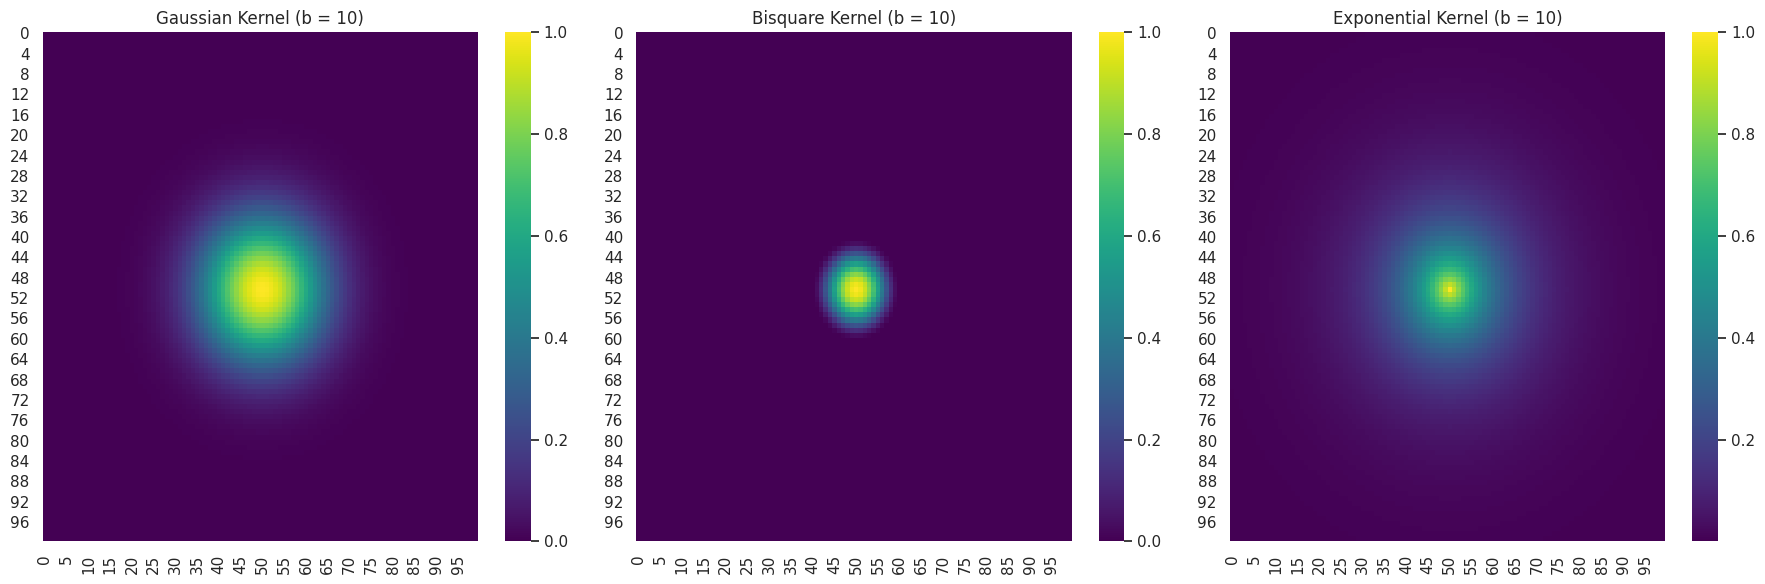
\includegraphics[width=0.85\linewidth]{gfx/m6l3_img004.png}
\par\smallskip{\small \textbf{Hình:} Hàm nhân (kernel) theo khoảng cách Euclid, băng thông 10.}
\end{figure}

\begin{figure}[H]
\centering
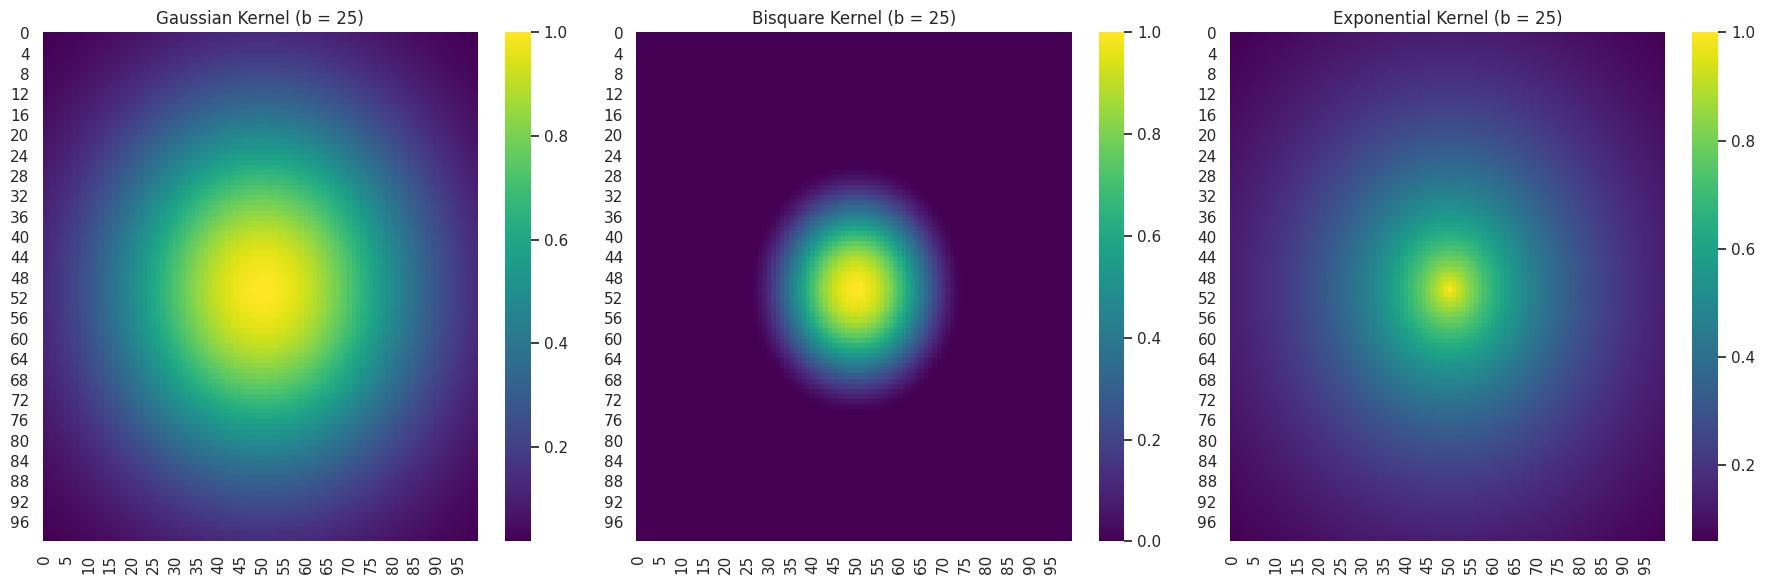
\includegraphics[width=0.85\linewidth]{gfx/m6l3_img005.png}
\par\smallskip{\small \textbf{Hình:} Hàm nhân (kernel) theo khoảng cách Euclid, băng thông 25.}
\end{figure}

\begin{figure}[H]
\centering
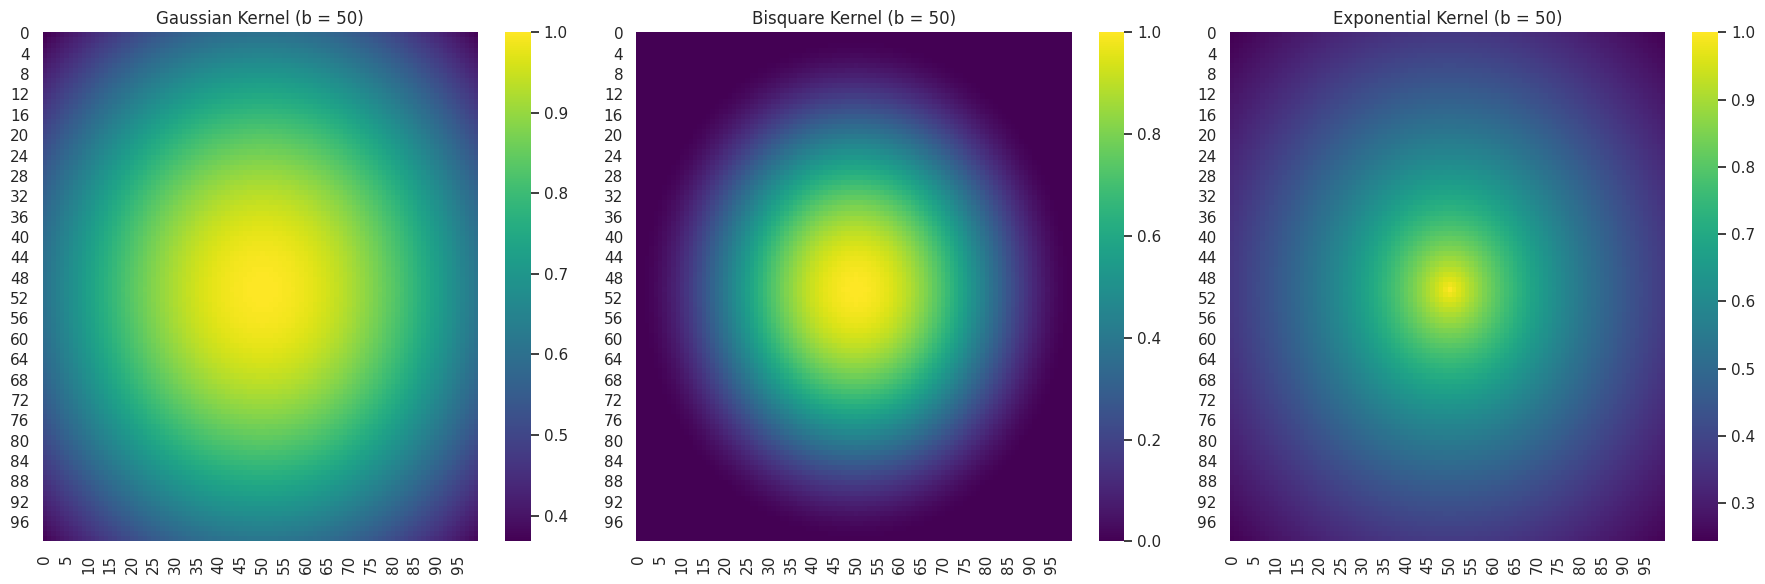
\includegraphics[width=0.85\linewidth]{gfx/m6l3_img006.png}
\par\smallskip{\small \textbf{Hình:} Hàm nhân (kernel) theo khoảng cách Euclid, băng thông 50.}
\end{figure}

Ở Hình 1 và 2, ta thấy tác động của băng thông lên việc chọn vùng lân cận: băng thông tăng thì vùng dùng trong hồi quy cục bộ cũng rộng ra. Hình dạng vùng cũng khác nhau theo từng thước đo khoảng cách. Quan trọng hơn, các hình làm rõ sự khác biệt giữa các hàm nhân:

\begin{itemize}
\item
  Gaussian: suy giảm dần và mượt, bắt đầu từ điểm quan tâm
\item
  Bisquare: cắt đột ngột, xác định rõ biên ảnh hưởng
\item
  Exponential: suy giảm nhanh nhưng có đuôi dài phản ánh các tác động ở khoảng cách xa
\end{itemize}

\section{Ứng dụng hồi quy trọng số địa lý (GWR)}

Trong phần này, chúng ta áp dụng những gì đã học về GWR ở phần trước vào dữ liệu thực tế.

\subsection{Nhập nguồn dữ liệu}

Ví dụ sử dụng dữ liệu cho thuê Airbnb tại khu Prenzlauer Berg (Prenz) ở Berlin, Đức (Oshan et al.). Prenz là điểm đến du lịch nổi tiếng, có nhiều lựa chọn ăn uống, nghệ thuật và đời sống về đêm. Dữ liệu được dùng để tìm hiểu các yếu tố chính quyết định giá thuê Airbnb trong khu vực này. Bộ dữ liệu có sẵn qua gói Python libpysal, nên cần cài gói này trước. Gói thứ hai cần cài là mgwr, gói Python để chạy GWR. Cài hai gói như sau.

\begin{lstlisting}[language=Python,escapeinside={(*@}{@*)}]
pip install libpysal
\end{lstlisting}

\begin{lstlisting}[language=Python,escapeinside={(*@}{@*)}]
pip install mgwr
\end{lstlisting}

Tiếp theo, nhập các gói Python cần thiết cho ứng dụng này.

\begin{lstlisting}[language=Python,escapeinside={(*@}{@*)}]
import pandas as pd
import libpysal as ps
from libpysal.examples import available
from libpysal.examples import load_example
from libpysal.examples import get_path
from mgwr.gwr import GWR, MGWR
from mgwr.sel_bw import Sel_BW
from mgwr.utils import compare_surfaces, truncate_colormap
import geopandas as gp
import folium
\end{lstlisting}

Pysal chứa nhiều bộ dữ liệu mẫu cho phân tích không gian; chi tiết xem tại \href{https://pysal.org/notebooks/lib/libpysal/Example_Datasets.html\#Datasets-for-use-with-libpysal}{Pysal Example Data}. Hàm sau cho phép xem danh sách các bộ dữ liệu mẫu của Pysal.

\begin{lstlisting}[language=Python,escapeinside={(*@}{@*)}]
# Check available datasets on Pysal
available()
\end{lstlisting}

Output:

\begin{lstlisting}[escapeinside={(*@}{@*)}]
         Name                                        Description  Installed
0       10740  Albuquerque, New Mexico, Census 2000 Tract Dat...       True
1      AirBnB  Airbnb rentals, socioeconomics, and crime in C...      False
2     Atlanta       Atlanta, GA region homicide counts and rates      False
3   Baltimore          Baltimore house sales prices and hedonics      False
4   Bostonhsg               Boston housing and neighborhood data      False
..        ...                                                ...        ...
94        taz           Traffic Analysis Zones in So. California      False
95      tokyo                               Tokyo Mortality data       True
96  us_income  Per-capita income for the lower 48 US states 1...       True
97   virginia                        Virginia counties shapefile       True
98       wmat          Datasets used for spatial weights testing       True

[99 rows x 3 columns]
\end{lstlisting}

Tiếp theo, tải bộ dữ liệu Prenz. Trên Pysal bộ này có tên "Berlin", nên đoạn mã dưới đây tải bộ dữ liệu Berlin.

\begin{lstlisting}[language=Python,escapeinside={(*@}{@*)}]
#Download Prenz (Berlin) dataset from Pysal
berlin = load_example('berlin')

# Check if the dataset is intalled and ready for analysis
berlin.installed
\end{lstlisting}

Output:

\begin{lstlisting}[escapeinside={(*@}{@*)}]
True
\end{lstlisting}

\subsection{Trực quan hóa dữ liệu}

Bộ dữ liệu đã được cài đặt. Hãy xem bên trong có gì.

\begin{lstlisting}[language=Python,escapeinside={(*@}{@*)}]
# Check file lists from the installed dataset
berlin.get_file_list()
\end{lstlisting}

Output:

\begin{lstlisting}[escapeinside={(*@}{@*)}]
['/usr/local/lib/python3.10/dist-packages/libpysal/examples/berlin/prenzlauer.zip',
 '/usr/local/lib/python3.10/dist-packages/libpysal/examples/berlin/README.md',
 '/usr/local/lib/python3.10/dist-packages/libpysal/examples/berlin/prenz_bound.zip']
\end{lstlisting}

Trong danh sách tệp, "prenzlauer.zip" chứa dữ liệu cần phân tích, còn "prenz\_bound.zip" dùng để vẽ ranh giới khu Prenz. Ta dùng hàm "get\_path" của Pysal và hàm "read.file" của geopandas để chuyển hai tệp này thành geo-dataframe.

\begin{lstlisting}[language=Python,escapeinside={(*@}{@*)}]
# Convert two zipped files to geo dataframes
prenz = gp.read_file(berlin.get_path('prenzlauer.zip'))
prenz_bound = gp.read_file(berlin.get_path('prenz_bound.zip'))
\end{lstlisting}

Kiểm tra lại kiểu của hai tệp đã chuyển đổi.

\begin{lstlisting}[language=Python,escapeinside={(*@}{@*)}]
# Check the type of Prenz dataset
type(prenz)
\end{lstlisting}

Output:

\begin{lstlisting}[escapeinside={(*@}{@*)}]
geopandas.geodataframe.GeoDataFrame
\end{lstlisting}

\begin{lstlisting}[language=Python,escapeinside={(*@}{@*)}]
# Check the type of Prenz_bound dataset
type(prenz)
\end{lstlisting}

Output:

\begin{lstlisting}[escapeinside={(*@}{@*)}]
geopandas.geodataframe.GeoDataFrame
\end{lstlisting}

Cả hai đều là bộ dữ liệu địa lý. Xem nội dung của chúng.

\begin{lstlisting}[language=Python,escapeinside={(*@}{@*)}]
prenz.head()
\end{lstlisting}

Output:

\begin{lstlisting}[escapeinside={(*@}{@*)}]
   accommodat  review_sco  bedrooms  bathrooms  beds  price             X  \
0           2       100.0       1.0        1.0   1.0   35.0  1.494450e+06   
1           2        90.0       1.0        1.0   1.0   23.0  1.494354e+06   
2           2        93.0       1.0        1.0   1.0   38.0  1.494406e+06   
3           2       100.0       1.0        1.0   1.0   50.0  1.494271e+06   
4           2       100.0       1.0        1.0   1.0   80.0  1.493982e+06   

              Y                         geometry  
0  6.899036e+06  POINT (1494450.105 6899036.141)  
1  6.899121e+06  POINT (1494353.555 6899120.594)  
2  6.898809e+06  POINT (1494405.897 6898808.518)  
3  6.898655e+06  POINT (1494270.517 6898655.223)  
4  6.899397e+06  POINT (1493982.078 6899397.385)
\end{lstlisting}

\begin{lstlisting}[language=Python,escapeinside={(*@}{@*)}]
# Find out number of rental properties in the dataset
len(prenz)
\end{lstlisting}

Output:

\begin{lstlisting}[escapeinside={(*@}{@*)}]
2203
\end{lstlisting}

Đoạn mã trên hiển thị năm dòng đầu của dữ liệu Prenz và cho biết bộ dữ liệu có 2.203 căn nhà cho thuê. Mô tả các biến:

\begin{itemize}
\item
  \textbf{accommodat}: Số khách tối đa căn nhà có thể tiếp nhận
\item
  \textbf{review\_sco}: Điểm đánh giá tích lũy từ khách gần nhất đã lưu trú
\item
  \textbf{bedrooms}: Số phòng ngủ
\item
  \textbf{bathrooms}: Số phòng tắm
\item
  \textbf{beds}: Số giường
\item
  \textbf{price}: Giá thuê
\item
  \textbf{X}: Vĩ độ của vị trí căn nhà
\item
  \textbf{Y}: Kinh độ của vị trí căn nhà
\item
  \textbf{geometry}: Vị trí địa lý của căn nhà
\end{itemize}

Bài trước đã nêu đặc điểm chính của bộ dữ liệu địa lý là có biến địa lý "geometry" cung cấp thông tin vị trí cho mỗi đặc trưng. Vì vị trí nhà cho thuê là dữ liệu điểm, ta chỉ có một cặp tọa độ gồm vĩ độ và kinh độ.

Tiếp theo, xem bộ dữ liệu địa lý prenz\_bound.

\begin{lstlisting}[language=Python,escapeinside={(*@}{@*)}]
prenz_bound.head()
\end{lstlisting}

Output:

\begin{lstlisting}[escapeinside={(*@}{@*)}]
       neighbourh                                           geometry
0  Helmholtzplatz  POLYGON ((1496989.669 6899662.266, 1497008.148...
\end{lstlisting}

Như đã giải thích, prenz\_bound cung cấp thông tin địa lý để vẽ ranh giới khu Prenz. Bộ dữ liệu này gồm tọa độ của nhiều điểm trên bản đồ; nối các điểm đó lại sẽ tạo thành một vùng (đa giác), nên prenz\_bound chỉ có một dòng dữ liệu.

Trước khi phân tích, hãy vẽ vị trí các căn nhà cho thuê lên bản đồ.

\begin{lstlisting}[language=Python,escapeinside={(*@}{@*)}]
# Draw Rental Properties of Prenz on a map

# First, create a basemap
map = folium.Map(location=[52.542986,13.427986], zoom_start=13.5, control_scale=True)

# Then add the Prenz neighborhood borders to the map
folium.GeoJson(prenz_bound).add_to(map)

# Then add the Airbnb rental locations to the map. We will use a red dot to represent the location of one airbnb rental.
folium.GeoJson(prenz,
               marker=folium.Circle(radius=10, fill_color="red", fill_opacity=0.4, color="red", weight=1)).add_to(map)

map
\end{lstlisting}

Output:

\begin{lstlisting}[escapeinside={(*@}{@*)}]
<folium.folium.Map at 0x7e6897fc5000>
\end{lstlisting}

\subsection{Chạy mô hình GWR}

Trong phần này, ta dùng dữ liệu Prenz để xây dựng mô hình định giá GWR bằng gói Python mgwr. Biến phụ thuộc là logarit của giá, nhằm hiệu chỉnh độ lệch (skewness) của dữ liệu giá. Ba biến độc lập là điểm đánh giá, số khách và số phòng tắm. Phương trình tuyến tính có dạng sau.

\textbf{log(price) = hệ số chặn + điểm đánh giá + số khách + số phòng tắm}

Ta cũng tạo một biến danh sách chứa thông tin của hai biến \(u\) và \(v\) đã mô tả ở phần 1.

\begin{lstlisting}[language=Python,escapeinside={(*@}{@*)}]
#Create variables for Berlin GWR pricing model
#Take the logarithm of the price variable to correct for skewing
b_y = np.log(prenz['price'].values.reshape((-1, 1)))
b_X = prenz[['review_sco','accommodat','bathrooms']].values
u = prenz['X']
v = prenz['Y']
b_coords = list(zip(u, v))
\end{lstlisting}

Sau khi tạo xong các biến cần cho mô hình, bước tiếp theo là xác định tham số băng thông (bandwidth).

Gói mgwr cung cấp hàm Sel\_BW để tìm băng thông tối ưu. Ta dùng quy trình tối ưu hóa và tiêu chí khớp mô hình mặc định của Sel\_BW. Mặc định là hàm nhân (kernel) bisquare và khoảng cách Euclid. Chọn kernel bisquare vì nó gán trọng số 0 cho các vị trí ở xa, trong khi kernel Gaussian và hàm mũ luôn gán trọng số khác 0 cho các vị trí ở xa.

Sau đó, Sel\_BW dùng phương pháp tìm kiếm mặc định dựa trên AIC hiệu chỉnh (AICc) để tìm băng thông tối ưu. \textbf{AIC hiệu chỉnh (AICc)} là một dạng AIC đặc biệt dùng cho phân tích không gian. AICc có thành phần phạt đối với băng thông nhỏ, vì băng thông nhỏ làm mô hình phức tạp hơn.

Bây giờ ta tìm băng thông cho mô hình.

\begin{lstlisting}[language=Python,escapeinside={(*@}{@*)}]
#Find bandwidth parameter
selector = Sel_BW(b_coords, b_y, b_X)
bw = selector.search()
print(bw)
\end{lstlisting}

Output:

\begin{lstlisting}[escapeinside={(*@}{@*)}]
192.0
\end{lstlisting}

Có băng thông rồi, ta dùng nó làm đầu vào để xây dựng mô hình GWR.

\begin{lstlisting}[language=Python,escapeinside={(*@}{@*)}]
# Build a GWR model and print out model summary
gwr_model = GWR(b_coords, b_y, b_X, bw)
gwr_results = gwr_model.fit()
gwr_results.summary()
\end{lstlisting}

Kết quả hồi quy toàn cục trong bản tóm tắt trên là kết quả mô hình OLS cho dữ liệu Prenz. Nó được dùng làm mô hình chuẩn so sánh (benchmark) với mô hình GWR. Kết quả OLS gồm phần tóm tắt mô hình thông thường mà ta đã quen thuộc.

\subsection{Xem xét kết quả mô hình}

Khối tiếp theo của phần tóm tắt là kết quả mô hình GWR, trước hết cho biết hàm nhân (kernel) bisquare và băng thông (bandwidth) 192 được chọn cho mô hình này, cùng nhiều thông tin chẩn đoán mô hình. Chẳng hạn, R\textsuperscript{2} hiệu chỉnh của mô hình OLS là 0,271 trong khi của mô hình GWR là 0,391; như vậy GWR phù hợp dữ liệu tốt hơn OLS.

Tiếp theo là kết quả ước lượng tham số. Trong mô hình GWR, mỗi vị trí có một bộ ước lượng tham số cho các biến độc lập; ở đây mỗi biến độc lập có 2.203 ước lượng tham số. Trong phần tóm tắt trên, X0 là hệ số chặn, X1 là điểm đánh giá, X2 là số khách được phục vụ, X3 là số phòng tắm. Vì vậy phần tóm tắt cho biết trung bình, độ lệch chuẩn, giá trị nhỏ nhất, trung vị và lớn nhất của các ước lượng tham số của từng biến độc lập. Để xem chi tiết, ta dùng mã Python sau, hiển thị bộ tham số ước lượng cho từng vị trí; dưới đây là năm vị trí đầu tiên.

\begin{lstlisting}[language=Python,escapeinside={(*@}{@*)}]
# Show estimated parameters for
gwr_results.params[0:5]
\end{lstlisting}

Output:

\begin{lstlisting}[escapeinside={(*@}{@*)}]
array([[ 3.30479996e+00,  1.61014298e-03,  2.06243405e-01,
        -2.67321919e-02],
       [ 3.43635569e+00, -4.51930353e-04,  1.95844944e-01,
         5.37474550e-02],
       [ 3.27912291e+00,  2.92768647e-03,  2.12363255e-01,
        -8.10919052e-02],
       [ 2.88779932e+00,  5.06056110e-03,  2.45744327e-01,
        4.65164479e-02],
       [ 2.89309002e+00,  3.06784769e-03,  1.67282256e-01,
         3.42487452e-01]])
\end{lstlisting}

GWR xây dựng một hồi quy cho mỗi vị trí nên mỗi vị trí cũng có R\textsuperscript{2} riêng. Dưới đây là R\textsuperscript{2} của 10 vị trí đầu tiên.

\begin{lstlisting}[language=Python,escapeinside={(*@}{@*)}]
gwr_results.localR2[0:10]
\end{lstlisting}

Output:

\begin{lstlisting}[escapeinside={(*@}{@*)}]
array([[0.39583113],
       [0.41660429],
       [0.35650484],
       [0.43641022],
       [0.44784271],
       [0.41771337],
       [0.42162229],
       [0.41387561],
       [0.36649332],
       [0.46269692]])
\end{lstlisting}

Ta cũng có thể vẽ biểu đồ R\textsuperscript{2} của mọi vị trí.

\begin{lstlisting}[language=Python,escapeinside={(*@}{@*)}]
#Show local model fit (R squared) for all locations
prenz['R2'] = gwr_results.localR2
prenz.plot('R2', legend = True)
ax = plt.gca()
ax.get_xaxis().set_visible(False)
ax.get_yaxis().set_visible(False)
plt.title("Local Model Fit")
plt.show()
\end{lstlisting}

\begin{figure}[H]
\centering
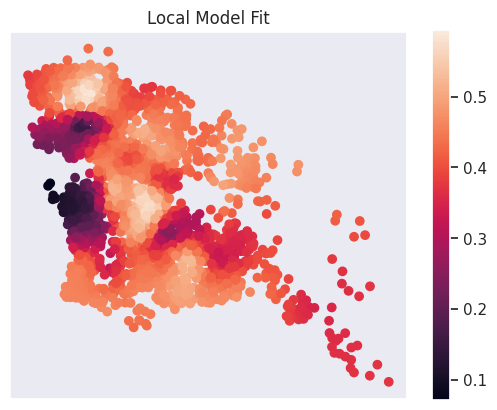
\includegraphics[width=0.85\linewidth]{gfx/m6l3_img007.png}
\par\smallskip{\small \textbf{Hình:} Độ khớp của mô hình cục bộ (Local Model Fit) trên bản đồ.}
\end{figure}

Từ biểu đồ "Local Model Fit", hai vùng sáng bên trái có nhiều vị trí nhất với R\textsuperscript{2} trên 0,5. Tuy nhiên, ở khu vực lệch trái so với trung tâm của khu phố, nhiều vị trí có R\textsuperscript{2} dưới 0,2.

\subsection{Minh họa tính các tham số GWR bằng đại số tuyến tính}

Phần này trình bày cách dùng đại số tuyến tính để thu được các ước lượng tham số của GWR. Trước hết, ta nhắc lại bộ ước lượng GWR cho các ước lượng tham số cục bộ tại vị trí \(i\).

\[\hat{\beta}(i)=\left[ X'W(i)X \right]^{-1}X'W(i)y\]

Ta dùng công thức trên để tính ước lượng tham số cho vị trí 1 (i bằng 0 vì Python đánh chỉ số từ 0). Vì ma trận trọng số được suy ra từ phương pháp tìm kiếm tối ưu, ta lấy trực tiếp từ kết quả mô hình để làm đầu vào.

\begin{lstlisting}[language=Python,escapeinside={(*@}{@*)}]
#Pull the information of weight matrix of location 1 from GWR model result
W_1 = gwr_results.W[0]
W_matrix = np.diag(W_1)
\end{lstlisting}

Tiếp theo, tạo ma trận \(X\): ma trận có các biến độc lập làm cột, kèm một cột toàn số 1 để ước lượng hệ số chặn.

\begin{lstlisting}[language=Python,escapeinside={(*@}{@*)}]
# Create X matrix with additional column of all 1s.
b_X_1 = np.hstack([np.ones((b_X.shape[0], 1)), b_X])
\end{lstlisting}

Tính trước ma trận nghịch đảo \(\left[ X'W(i)X \right]^{-1}\) trong công thức.

\begin{lstlisting}[language=Python,escapeinside={(*@}{@*)}]
inverse_matrix = np.linalg.inv(b_X_1.T@W_matrix@b_X_1)
\end{lstlisting}

Tiếp theo, tính ước lượng tham số cho vị trí 1.

\begin{lstlisting}[language=Python,escapeinside={(*@}{@*)}]
beta_1 = inverse_matrix@b_X_1.T@W_matrix@b_y
beta_1
\end{lstlisting}

Output:

\begin{lstlisting}[escapeinside={(*@}{@*)}]
array([[ 3.30479996e+00],
       [ 1.61014298e-03],
       [ 2.06243405e-01],
       [-2.67321919e-02]])
\end{lstlisting}

So sánh với kết quả của mô hình GWR.

\begin{lstlisting}[language=Python,escapeinside={(*@}{@*)}]
gwr_results.params[0]
\end{lstlisting}

Output:

\begin{lstlisting}[escapeinside={(*@}{@*)}]
array([ 3.30479996e+00,  1.61014298e-03,  2.06243405e-01, -2.67321919e-02])
\end{lstlisting}

Hai kết quả trùng khớp, cho thấy đại số tuyến tính được áp dụng thế nào vào việc tính mô hình GWR.

\section{Kết luận}

Bài học này trình bày lý thuyết về hồi quy trọng số địa lý (GWR), gồm định nghĩa và các khái niệm chính, đặc biệt là các phương pháp hàm nhân (kernel) và cách tính khoảng cách cho GWR, cũng như cách tính băng thông (bandwidth) của mô hình. Tiếp đó, chúng ta dùng một bộ dữ liệu thực tế để minh họa cách xây dựng mô hình GWR và so sánh kết quả với mô hình OLS truyền thống. Cuối cùng, chúng ta chỉ ra cách dùng đại số tuyến tính để suy ra các ước lượng tham số của mô hình GWR.
